\chapter{Testy systemu}
\section{Lokalizowanie użytkownika}
Celem testów jest zbadanie jakości wyznaczonej przez system lokalizacji użytkownika w rzeczywistym środowisku.\\
Przygotowany został jeden telefon z aplikacją mobilną, który pełnił rolę odbiornika oraz 3 transmitery Wifi (1 router i 2 access-pointy). Obszar działania miał wielkość 10 metrów na 7,2 metra. Jako punkt 'zerowy' (0,0,0) został przyjęty lewy górny róg. 
\begin{figure}[H]			
	\centering
	\caption{Schemat modelu do testów lokalizacji}
	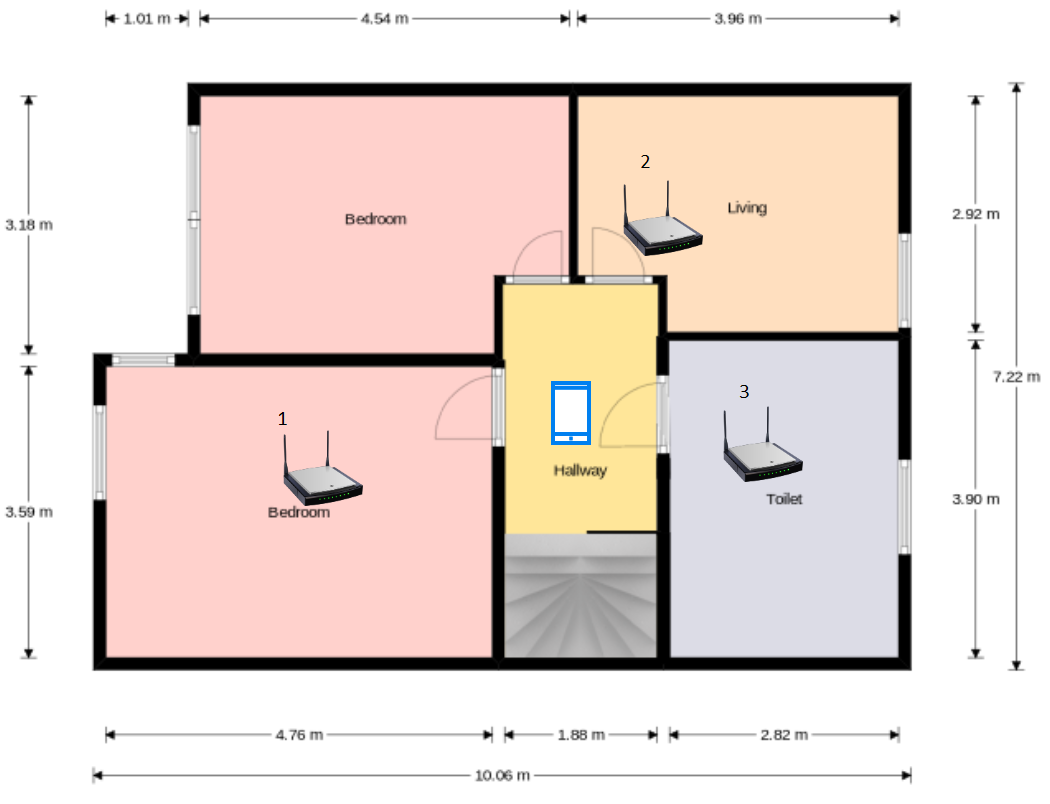
\includegraphics[width=1.0\textwidth]{plan}
\end{figure}
Dla tak przyjętych założeń, kolejne urządzenia mają współrzędne:
\begin{itemize}
	\item transmiter nr 1 - współrzędne (2.5, 4.75, 0.1)
	\item transmiter nr 2 - współrzędne (7.5, 1.25, 0.0)
	\item transmiter nr 3 - współrzędne (8.25, 4.5, 0.0)
	\item odbiornik - współrzędne (6.0, 4.25, 0.0)
\end{itemize}
Wykonana została seria 7 powtórzeń, podczas których aplikacja wysłała informacje o odbieranych przez nią siłach sygnałów, a serwer, po ich odebraniu, wyznaczył lokalizację. Błąd względny był obliczany w odniesieniu do założonego, akceptowalnego błędu podczas lokalizacji - 0.5 metra.
 \begin{center}
	\begin{minipage}{\linewidth}
		\begin{tabular}{|c|c|c|c|>{\centering} p{6cm}|c|}
			\hline 
			Pomiar & X & Y & Z & Dystans między rzeczywistą pozycją, a obliczoną (m) & Błąd względny (\%)\\ 
			\hline 
			1 & 6.11 & 3.78 & -0.12 & 0.5 & 100\\ 
			\hline 
			2 & 5.65 & 3.24 & 0.06 & 1.07 & 214 \\ 
			\hline 
			3 & 6.53 & 3.90 & 0.51 & 0.81 & 162 \\ 
			\hline 
			4 & 4.87 & 2.53 & -0.1 & 2.06 & 412 \\ 
			\hline 
			5 & 6.98 & 2.23 & -0.04 & 2.25 & 450 \\
			\hline
			6 & 5.09 & 3.90 & 0.01 & 0.98 & 196 \\
			\hline
			7 & 7.44 & 3.50 & -0.22 & 1.64 & 328 \\
			\hline 
		\end{tabular} 
	\end{minipage} 
\end{center}
Lokalizacja została również zarejestrowana przez aplikację administracyjną (na zielono zaznaczono faktyczną pozycję użytkownika).
\begin{figure}[H]			
	\centering
	\caption{Widok mapy w aplikacji klienckiej}
	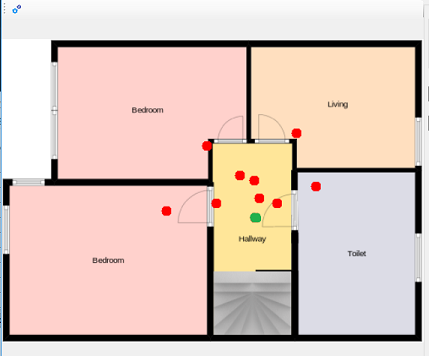
\includegraphics{eksperyment_lokalizacja}
\end{figure}
Z eksperymentu wynika, że określanie lokalizacji na podstawie siły sygnału wysyłanego przez transmiter ma niższą skuteczność niż oczekiwałem na początku. W ramach rozwijania aplikacji w przyszłości, warto znaleźć lepszy sposób na dokładniejsze określanie odległości odbiornika od transmiterów.
\section{Monitorowanie i konfiguracja systemu}
Dodatkowo, przed zarejestrowaniem lokalizacji użytkownika w poprzednim eksperymencie, do systemu zostało dodane jedno urządzenie oświetleniowe. Jego zasięg został ustawiony na 0.75 metra, a lokalizacja na (6.1, 4.4, 0). Urządzeniu został również przypisany moduł obsługi eventów - ImportantUserFirstContr - tak, aby światło zostało ustawione na wartość maksymalną w momencie, jak w okolicy zostanie zarejestrowana obecność telefonu z aplikacją mobilną. Użytkownikowi, który brał udział w teście, została nadana najwyższa waga.\\
W momencie zarejestrowania lokalizacji o współrzędnych (6.11, 3.78, -0.12), odległość od urządzenia wynosiła 0.63 metra, co oznacza, że znalazła się w zasięgu urządzenia. Spowodowało to wysłanie przez serwer do urządzenia parametru o wartości równej maksymalnej sile światła (w tym wypadku wynosiło to 80\%).\\
Dodatkowo, w momencie wywołania się modułu czasowego, jako lokalizację przynależące do urządzenia zostały zakwalifikowane dwie współrzędne, co spowodowało, że serwer wysłał parametr równy 33\%, ponieważ:
\begin{equation}
P_{ustalona} = (P_{max} - P_{min}) * \frac{N_{blisk}}{N_{ogół}} + P_{min} = (80 - 20) * \frac{2}{9} + 20 = 33,3
\end{equation}
\begin{figure}[H]			
	\centering
	\caption{Wizualne przedstawienie zasięgu urządzenia}
	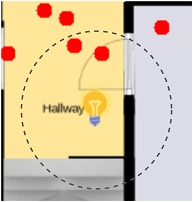
\includegraphics{dzialanie_urzadze}
\end{figure}
\section{Podsumowanie}
Celem pracy było stworzenie systemu, który określa położenie użytkownika w trzech wymiarach na podstawie siły sygnału znanych routerów, stałych urządzeń Bluetooth (np Beaconów) oraz dynamicznie zmieniających się sił sygnałów Bluetooth innych użytkowników systemu. Obliczone lokalizacje miały być przechowywane oraz przedstawiane na mapie budynku w sposób łatwy do analizy. Dodatkowo, celem było opracowanie algorytmu, który na podstawie określonych warunków oraz mapy przepływu zarządza wybranymi urządzeniami podłączonymi do systemu.\\
W ramach projektu został zaimplementowany pełny moduł do lokalizacji użytkowników. Dane zbierane z aplikacji mobilnych są przedstawiane jako trójwymiarowy model, w której odległość między transmiterem, a odbiornikiem została opisana jako probabilistyczna funkcja Gaussa. Mierzenie dystansu pomiędzy urządzeniami opiera się na obliczaniu mocy zaniku siły sygnałów Bluetooth oraz Wifi, odbieranego przez urządzenia mobilne.\\
Aby system mógł lepiej określać lokalizację aplikacji mobilnych, przeprowadzone zostały testy technologii Bluetooth oraz Wifi. Ich celem było określenie, który z wyżej wymienionych sposobów komunikacji jest bardziej niezawodny oraz odporny na zakłócenia i odbicia. Niestety, ogólne testy całej aplikacji wykazały, że określanie odległości na podstawie RSSI nie jest wystarczająco dokładne, jednakże dobór lepszej metody może być uwzględniony podczas dalszego rozwoju aplikacji.\\
Dodatkowo, stworzona została aplikacja administracyjna, mająca możliwość zarządzania całym systemem oraz monitorowania lokalizacji użytkowników. Prezentowane przez nią dane pozwalają na analizę przepływu ludzi, a dzięki odpowiedniemu skonfigurowaniu, aplikacja serwerowa ma możliwość efektywnego sterowania zarejestrowanymi urządzeniami na podstawie odnotowanych lokalizacji użytkowników.\\
Aplikacja może być w przyszłości rozwijana w wielu różnych kierunkach. Po pierwsze, testy wykazały, że aby aplikacja mogła dokładnie wyznaczać lokalizację, potrzebne jest znalezienie innego sposobu określania odległości między transmiterem, a odbiornikiem. Dodatkowo, do aplikacji można dodawać nowe kategorie urządzeń oraz sposoby komunikacji z nimi. Aplikacja mobilna może zostać rozszerzona o moduł administracyjny, który pozwoli na sterowanie systemem z poziomu smartphona. Wreszcie, serwer może być rozwijany poprzez  stworzenie większej ilości modułów obsługi eventów.\\



